\documentclass{article}
\usepackage[utf8]{inputenc}
\usepackage{amsmath}
\usepackage{natbib}
\usepackage{graphicx}
%\usepackage{astrojournals} % Necesario para nombres de revistas en luis-ref.bib
\usepackage[spanish, es-minimal]{babel}
\bibliographystyle{apj}
\newcommand\U[1]{\ensuremath{\mathrm{#1}}}
\newcommand\K{\U{K}}
\newcommand\cm{\U{cm}}
\newcommand\AU{\U{AU}}
\newcommand\g{\U{g}}
\newcommand\msolagno{M_\odot\,\U{yr^{-1}}}

\newcommand\acre{\ensuremath{_{\mathrm{acre}}}}
\newcommand\eff{\ensuremath{_{\mathrm{eff}}}}
\newcommand\Ext{\ensuremath{_{\mathrm{Ext}}}}
\newcommand\Int{\ensuremath{_{\mathrm{Int}}}}
\newcommand\ha{\ensuremath{\mathrm{H}\alpha}}
\newcommand\nii{\ensuremath{\mathrm{[N\,II]}}}
\title{Capitulo 5: Resultados preliminares }

\author{
  Alumno: Luis Angel Gutiérrez Soto\\
  Tutor: Dr. William Henney
}

\begin{document}
\maketitle

\section{ Interacciones de los flujos externos e internos}
\label{sec:results}


Las observaciones de las que hemos hablado hasta el momento junto con los parámetros astrofísicos medidos nos han permitido esbosar algunos parámetros astrofísicos, con el objetivo de intentar compreder los fenómenos que en nuestros objetos están ocurriendo. En este orden de ideas hemos determinado la densidad en la cáscara del choque, la presión ram como en la cáscara y el flujo de momento, que es lo que veremos a continuación.

\subsection{Densidad}
\label{sec:density}

Dado que a partir de las observaciones hemos podido determinar el brillo superficial de \(\ha\) realizando un poco de fotometría como se puede apreciar previamente y además debido a que tenemos el camino de visión en la cáscara chocada (\(\Delta \zeta\))  hemos determinado la densidad de núcleos de Hidrógeno (\(n\)) especificamente en esa región (cáscara) para los diferentes objetos que entran en la muestra  usando la ecuación \ref{}. Hay que subrayar que hemos usado cómo distancia a la Nebulosa de Orión de  436 Pc (Odell \& Henney, 2008) para hacer las respectivas conversiones de unidades.\\ 

\begin{figure}
  \centering
   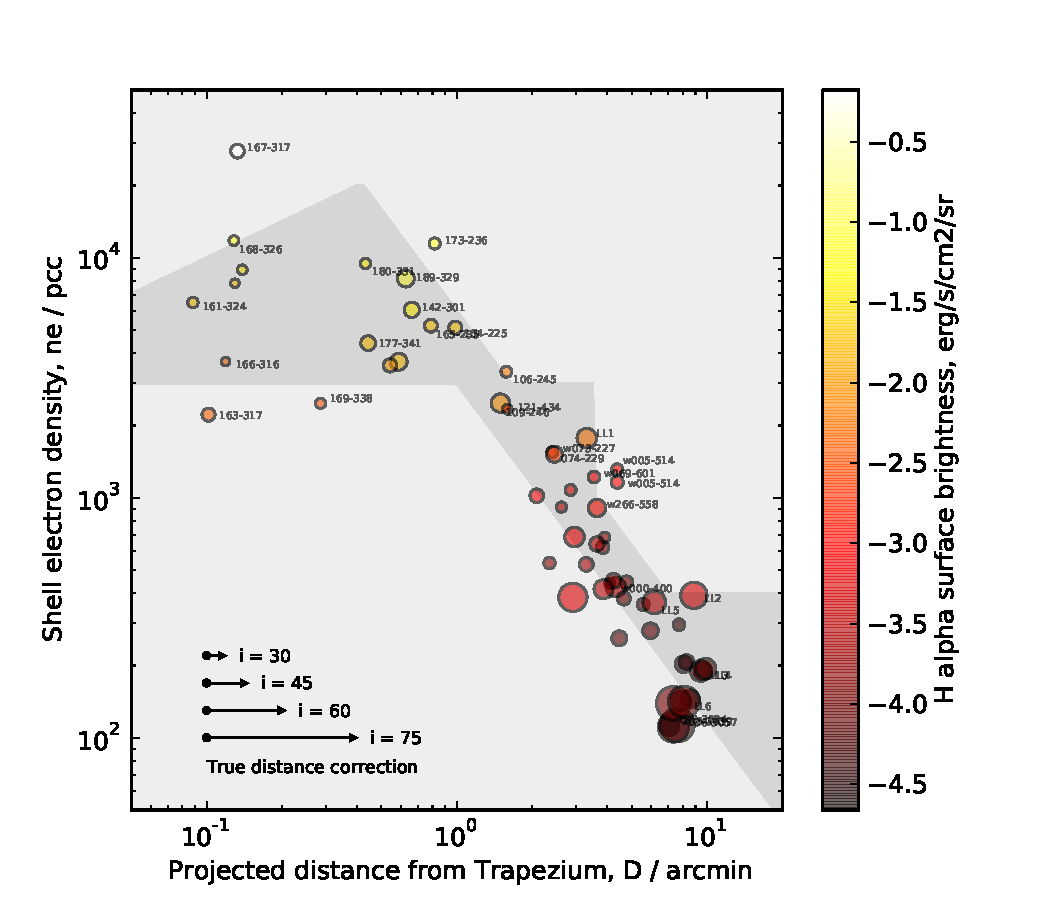
\includegraphics[width=\linewidth, clip]{luis-programas/will-nshell-vs-D.pdf}
  \caption{Densidad electrónica corregida por extinción en función de la distancia a \(\theta^1\ \text{Ori}\ \text{C}\) obtenida a partir de las observaciones, es decir del brillo superficial de \(\ha\) en la cáscara chocada. El tamaño de los puntos indica que tan grande es el camino de visión de la zona chocada si los comparamos entre si. Por otro lado el color de los puntos muestra que tan brillante es el objeto en cuestión al comparar con la barra que aparece a la derecha de la gráfica. }
  \label{fig:density}
\end{figure}

En la figura \ref{fig:density} se logra apreciar que los objetos que están más cercas de la estrella ionizante presentan una densidad electrónica mayor que los que se encuentran a las afueras de la nebulosa, generando con esto que las cáscaras en estas regiones sean mucho más radiativas.\\



\subsection{Presión hidrodinámica y presión térmica}
\label{sec:pressure}

A partir de la densidad electrónica y usando la ecuación ?? estimamos la presión térmica en la cáscara chocada y de la misma manera usando la ecuación ?? determinamos la presión ejercida por un viento estelar que a su vez es hipersónico.\\ 

\begin{figure}
  \centering
  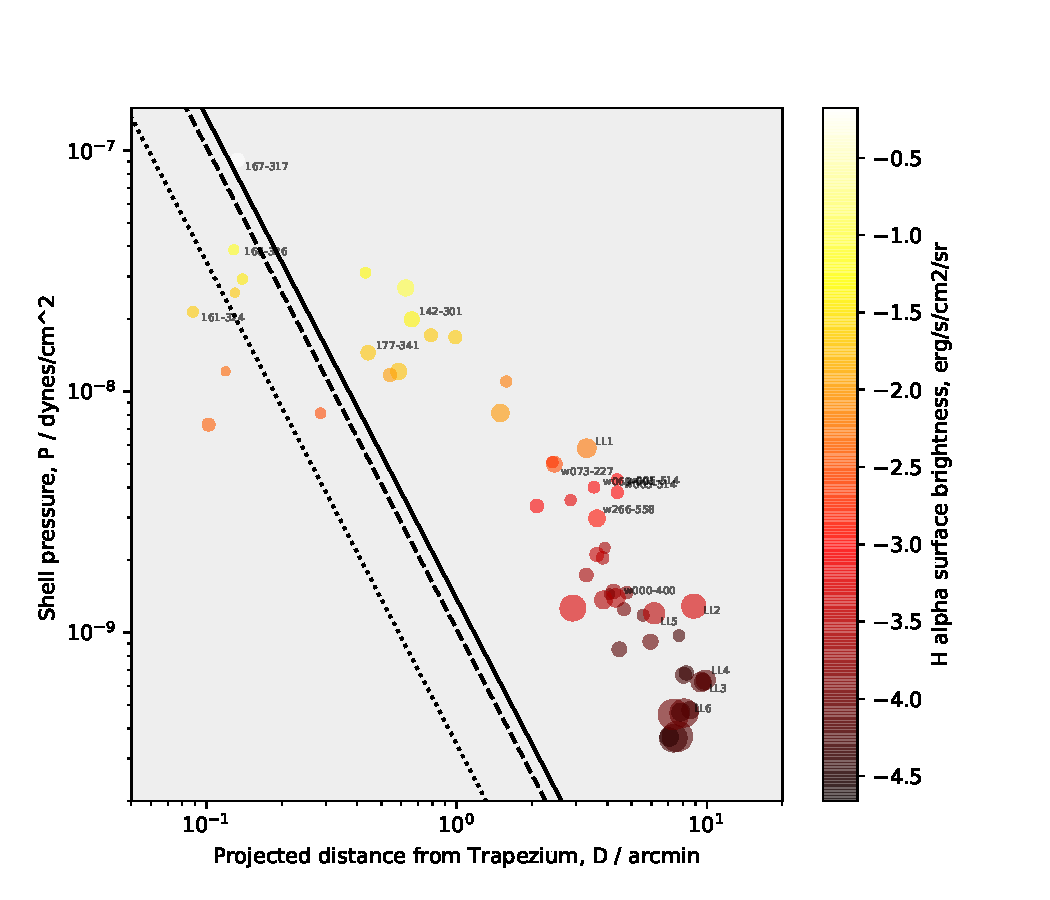
\includegraphics[width=\linewidth, clip]{luis-programas/will-Pshell-vs-D.pdf}
  \caption{Los puntos indican la presión térmica en la cáscara y la línea sólida hace referencia a la presión hidrodinámica generada por el viento estelar.}
 \label{fig:pressure}
\end{figure}

Así, la figura \ref{fig:pressure} muestra la presión térmica en la cáscara chocada, vemos que esta es mayor en los objetos que están adentro de la nebulosa y que además corresponde a una interacción del flujo interno con el viento estelar de la estrella ionizante.


\subsection{ Flujo de momento \(\dot{M}\text{V}\) }
\label{sec:momentum}

de la misma manera determinamos el flujo de momento interno para los objetos de nuestra muestra, usando para ello una tasa de perdida de masa de, una velocidad de y usando desde luego el radio del borde interno del choque. Es de notar que los objetos que no son proplyds y que están afuera de la nebulosa presentan fuertes vientos en cambio los que son proplydos y los que además pordrían serlos (no estamos seguros), presentan fuertes vientos pero estos van disminuyendo en la medida en que nos ubicamos en las regiones exteriones de la Nebulosa de Orión (ver figura \ref{fig:flow}).\\ 

\begin{figure}
  \centering
  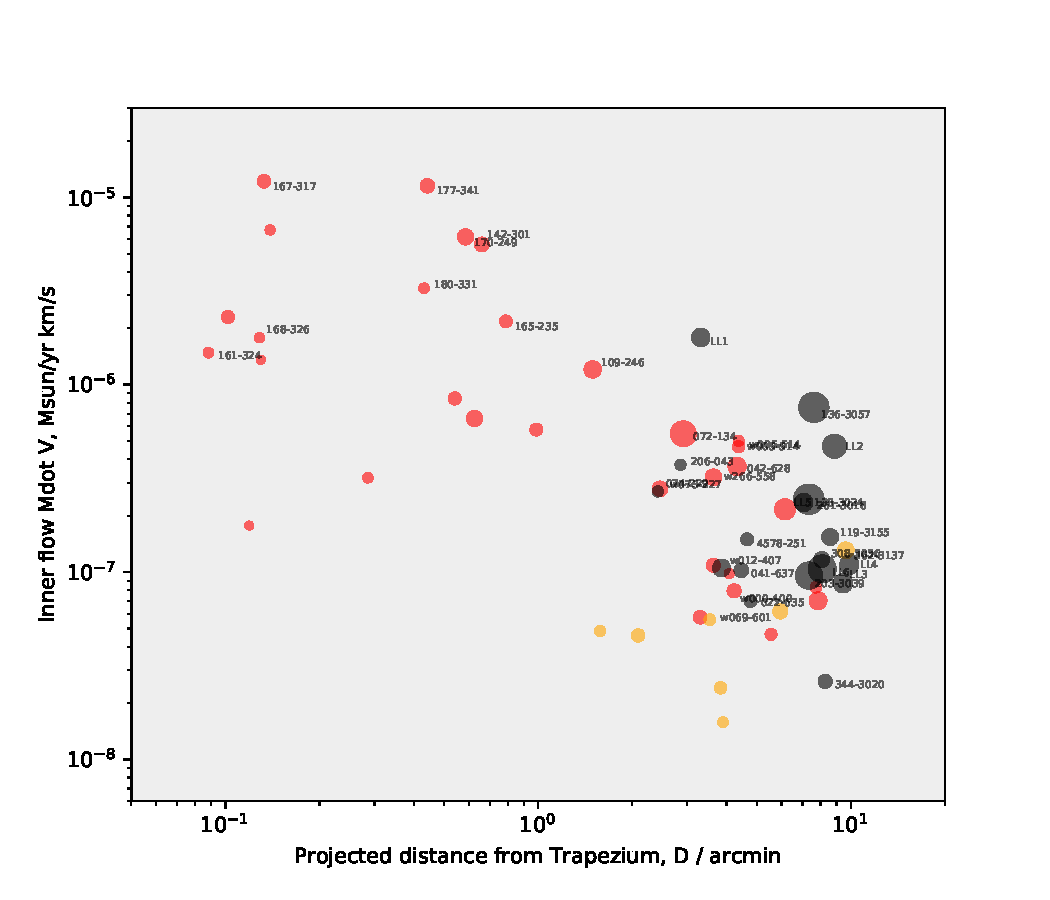
\includegraphics[width=\linewidth, clip]{luis-programas/will-MdotV-vs-D.pdf}
  \caption{Flujo de momento interno el color negro de los puntos indica que los objetos no son proplyds, los de color anaranjado podrían ser proplyds, y los de color rojo sabemos con certeza que son proplyds.}
 \label{fig:flow}
\end{figure}

La discrepancia entre las presion ram y las presiones internas en los objetos a distancias mayores, nos está diciendo que los choques de los mismos no se están generando a partir de la interacción con el viento de la estrella O del trapecio, si no que se debe a la interacción con el Flujo de Champaña

\end{document}
